\begin{figure}
  \begin{center}
    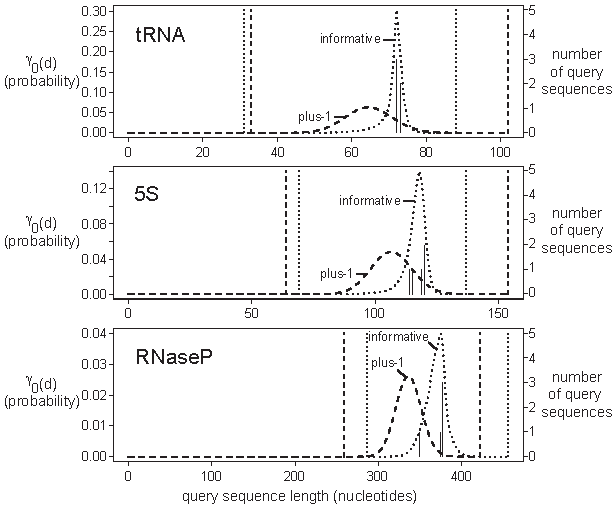
\includegraphics[width=6in,angle=0]{figs/bands}
    \caption{\textbf{Effect of transition priors on band calculation.}
      Predicted and actual target lengths are shown for three CMs
      built from alignments of five tRNA, 5S rRNA, and RNaseP
      sequences, which are about 75, 120, and 380 residues long,
      respectively.  Solid vertical lines are histogram bars of the
      actual lengths of the query sequences in each alignment,
      corresponding with the right vertical axis labels. Dashed and
      dotted curves show QDB calculations for $\gamma_0(d)$ for the
      root state of each model, for uninformative versus informative
      Dirichlet priors, respectively.  Dashed and dotted vertical
      lines show the band bounds ($\mbox{dmin}(0)$ (left) and
      $\mbox{dmax}(0)$ (right)) derived from the $\gamma_0(d)$
      distributions using $\beta = 10^{-7}$. The uninformative
      plus-one prior results in consistent underprediction of target
      sequence lengths, with a broad distribution. The new informative
      priors produce tighter distributions that are centered on the
      actual subsequence lengths. We observe the same result for all
      other states (data not shown).}
    \label{fig:bands}
  \end{center}
\end{figure}
